\chapter{Background Theory}
In this chapter, the theoretical background for the implementation of the \textit{CAD-integrated Topology Optimization} tool is presented. The chapter is divided into four sections: \emph{\nameref{sec:CADbackg}} (\autoref{sec:CADbackg}), \emph{\nameref{sec:TopOpt}} (\autoref{sec:TopOpt}), \emph{\nameref{sec:surfaceBackg}} (\autoref{sec:surfaceBackg}), and \emph{\nameref{sec:NURBS}} (\autoref{sec:NURBS}).
\label{chapter:Background}

\section{CAD overview}
\label{sec:CADbackg}
%interaction with it, programs, geometry represenations, datastructures, formats etc., maybe even history if we're overkill
\subsection{History of CAD}
Computer aided design (short: CAD) refers to the process of designing a product using a computer system. Before CAD applications were used, products were constructed using a sketch board. It was a challenge to incorporate changes in the construction drafts as well as to keep documentations up to date; hence, it was no surprise that CAD systems spread rapidly across all design development branches. Computer aided design is now irreplaceable used in architecture, mechanical, electrical and civil engineering.

Depending on the discipline different requirements are set on the virtual model. One may imagine that in a civil engineering model of a building a 2D floor plan is often sufficient; however in the design of a mechanical motor a 3D model is always necessary. Given these circumstances, various CAD software bundles evolved in the different disciplines with completely different modelling approaches. Besides the geometry representation parameters, such as material properties or manufacturing information, are stored. In order to move between different data structures standardized exchange interfaces are commonly used.
\subsection{Geometry representations}
In general, two different ways of describing a geometry are used in CAD systems: constructive solid geometry consisting of a set of primitive forms or storing the boundary of a part assuming that the interior is filled (BREP). Other approaches, such as a complete voxelised geometry are not common due to extensive memory consumption.
\subsubsection{Constructive solid geometry}
\begin{figure}
\centering
\includegraphics[width=0.5\textwidth]{Pictures/Csg_tree.png}
\caption{CSG object tree}
\label{fig:csg_tree}
\end{figure}
One way of representing a geometry in CAD is the approach of \emph{constructive solid geometry} (short: CSG). The basic idea is to start from a set of primitives, e.g. a sphere, cylinder and cube. Basic Boolean operations link these primitives towards a complex geometry. This procedure can be seen in figure \ref{fig:csg_tree}.

Key advantages of this format is the precise representation using very few storage memory. However, not all desired forms can be represented by CSG and hence, a second type of geometry description is needed. 
\subsubsection{Boundary representation}
A different kind of modelling approach is the so-called \emph{boundary representation}. Instead of storing the geometry information at every single point, \emph{BREP} formats only save the boundary surface of the body. The interior is assumed to be uniformly filled. Especially in big geometries this approach simplifies the model immensely to an extend that amounts of data are better to handle. Surfaces can be stored as tetrahedrons (see later STL files) or in NURBS patches.
Furthermore, holes in the body are possible by saving the surface normal of the boundary surface. 

By the boundary representation arbitrary geometries can be created. Data amounts to fulfill a certain precision are larger than by the csg representation, but BREP files are usually easier to work with. Beware, that unreal geometries can be created using BREP formats.
\subsection{Data exchange file formats}


\section{Topology Optimisation}
\label{sec:TopOpt}
%how the algorithms work, maybe what it can be used for
\subsection{Definition and motivation}
Topology Optimization describes the process of finding the optimal distribution of a limited amount of material for a given area or volume based on a predefined constraint/minimization problem. Possible optimization goals are for example:
\begin{itemize}
\item \textbf{Minimum compliance} which seeks to find the optimal distribution of material that returns the stiffest possible structure. The structure is thereby subjected to loads (forces) and supports (boundary conditions). By maximizing the stiffness, we minimize the compliance.
\item \textbf{Heat conduction} tries to optimize the domain of a conductive material with respect to conductivity for the purpose of heat transfer. This maximization problem is the same as minimizing the temperature gradient over the domain-- a poor conductor will create a large gradient.
\item \textbf{Mechanism synthesis}' objective is to obtain a device that can convert an input displacement in one location to an output displacement in another location. Topology Optimization hereby seeks the optimal design which maximizes the output force for a given input or, respectively, minimizes the input force for a given output.
\end{itemize}


As one can imagine by this short list of optimization goals, Topology Optimization has a wide field of possible applications. Hence, it has become a well established technology used by engineers in the fields of aeronautics, civil, materials, mechanical and structural optimization. Furthermore, the rising significance of 3D-printers in industry, the realisation of computed optimized designs is now much easier.

\subsection{Theory}
%Maybe a little theory here about how topology optimization actually works

\subsection{ToPy}
ToPy \cite{ToPy} is a python library/program, written by William Hunter and documented in \cite{Hunter2009}. It is based on the 99-line Matlab code by Sigmund's for minimum compliance. The program can optimize the three above named problem types, minimum compliance, heat conduction and mechanism synthesis-- in 2D as well as 3D. It uses available open source python software, as for example Pysparse and Numpy, leading to improved speed, porta- and scalability. The whole program is steered by an input file which-- with the help of the documentation-- is straightforward to use and easy to adapt. 

\subsection{Implementation}
In terms of our implementation, we use ToPy as a blackbox topology optimizer. This means, we launch the program with an input file based on our scenario, let ToPy run and proceed by working with the output of ToPy. The intention is to touch the solver itself as less as possible to be able to just plug in different solvers later on. Implementation-wise that means, that we wrote a program which takes as input a voxelized CAD design in, for example, stl-format and outputs a tpd-file which can be used by ToPy. Results of the process can be seen in figure \ref{fig: topyStar}. Here, a star was given as input from a stl-file. We fixed the voxels in the corners of the structure, while we set a load in the middle, pointing into the structure. As can be seen, the optimization process "cuts" away unnecessary material in-between the corners and even in the middle of the material and returns stiff structure for a minimal amount of material. (maybe a bit wishy washy here)
\begin{figure}
\centering
\begin{subfigure}{
  \includegraphics[width=.2\linewidth]{Pictures/TopOp/Star_Optimized0_Trans.png}}
\end{subfigure}%
\begin{subfigure}{
  \includegraphics[width=.2\linewidth]{Pictures/TopOp/Star_Optimized2_Trans.png}}
\end{subfigure}
\begin{subfigure}{
  \includegraphics[width=.2\linewidth]{Pictures/TopOp/Star_Optimized4_Trans.png}}
\end{subfigure}
\begin{subfigure}{
  \includegraphics[width=.2\linewidth]{Pictures/TopOp/Star_Optimized5_Trans.png}}
\end{subfigure}
\caption{Topology Optimization with minimum compliance of a star structure, given by an stl-file. The fixtures were applied in the corners of the star, while a load was set in the middle.}
\label{fig: topyStar}
\end{figure}


%section moved to implementation
%\section{From CAD to Voxels}
%%\subsection{Motivation}
%The goal of good design is to find the right balance between a set of parameters, which usually include efficiency, weight and aesthetics. For a long time, this process had been an ardous loop of minute modifications to the product, oscillating between the engineer and the designer. However, with the advent of Topology optimization (see \autoref{sec:TopOpt}) and additive manufacturing, it has been shrunk drastically to an efficient, compact task. In the previous section, we summarized the different ways of representing a design object digitally. On specifying the appropriate loads as boundary conditions on this object, one can choose their favourite topology optimization tool to compute the optimal dimensions and form.


The main hurdle with most state-of-the-art open source topology optimization tools is their input format, where many of them require input to be specified as a 3-dimensional voxel grid. Presence (or absence) of material in these voxels is defined by a boolean variable, and boundary conditions are imposed on the appropriate locations. %This section describes how we overcame this hurdle of converting CAD representations to voxelized input.



\section{From Voxels to a surface representation}
\label{sec:surfaceBackg}

\subsubsection{Dual Contouring}

\begin{frame}
	\frametitle{From Voxel to Mesh Geometry}
	Task:
	\begin{itemize}
	\item Extract isosurface from voxel information
	\item Algorithms: Marching Cubes, Dual Contouring, Extended Models
	\end{itemize}
	Steps: 
	\begin{enumerate}
		\item Locate the position of the vertex inside each cube which has at least one sign changing
		edge
		\item Join the vertices associated with four cubes sharing a common edge to form a quadrilateral face (quad)
	\end{enumerate}
	\begin{minipage}{0.49\textwidth}
	\only<1>{
	\begin{figure}	
	\centering
	\includegraphics[width=.35\textwidth]{Pictures/DC/MC1.png}\caption{Marching cube}
	\end{figure}}
	\only<2>{
		\begin{figure}	
		\centering
		\includegraphics[width=.35\textwidth]{Pictures/DC/MC2.png}\caption{Marching cube}
		\end{figure}}
	\only<3>{
		\begin{figure}	
		\centering
		\includegraphics[width=.35\textwidth]{Pictures/DC/MC3.png}\caption{Marching cube}
		\end{figure}}
			\only<4>{
				\begin{figure}	
				\centering
				\includegraphics[width=.35\textwidth]{Pictures/DC/MC4.png}\caption{Marching cube}
	\end{figure}}
	\end{minipage}
	\begin{minipage}{0.49\textwidth}
	\only<1>{
	\begin{figure}	
	\centering
	\includegraphics[width=.35\textwidth]{Pictures/DC/MC1.png}\caption{Dual Contouring}
	\end{figure}}
	\only<2>{
		\begin{figure}	
		\centering
		\includegraphics[width=.35\textwidth]{Pictures/DC/MC2.png}\caption{Dual Contouring}
		\end{figure}}
	\only<3>{
		\begin{figure}	
		\centering
		\includegraphics[width=.35\textwidth]{Pictures/DC/DC3.png}\caption{Dual Contouring}
		\end{figure}}
			\only<4>{
				\begin{figure}	
				\centering
				\includegraphics[width=.35\textwidth]{Pictures/DC/DC4.png}\caption{Dual Contouring}
	\end{figure}}
	
	\end{minipage}
%	\caption{Comparision of MC and DC for identical datasets. The vertices are created on the edges of the cubes for MC  and inside the cubes for DC. Please note that the sharp feature in the top right cube can only be reconstructed by DC. Figure from %\cite{FromVoxelsToPolygons}.
\end{frame}


\begin{frame}
	\frametitle{Two-grid Dual Contouring}
	\begin{overlayarea}{\textwidth}{0.9 \textheight}
	\begin{minipage}{0.45\textwidth}
	\begin{block}{\centering Coarse grid}
	\vspace{-0.5cm}
	\begin{figure}
	\includegraphics[scale=0.35]{Pictures/DC/DC_1_Coarse.pdf}
	\end{figure}
	\begin{itemize}
	\item Coarse quads used in \textcolor{red}{parametrization}
	\end{itemize}
	\end{block}
	\end{minipage}
	\hfill%
	\begin{minipage}{0.45\textwidth}
	\begin{block}{\centering Fine grid}
	\vspace{-0.5cm}
	\begin{figure}
	\includegraphics[scale=0.35]{Pictures/DC/DC_1_Fine.pdf}
	\end{figure}
	\begin{itemize}
	\item Fine vertices used for \textcolor{red}{projection}
	\end{itemize}
	\end{block}
	\end{minipage}
	\end{overlayarea}
\end{frame}

%\subsection{B--Spline}

\subsection{Projection and Parametrization}
\begin{frame}{Projection and Parametrization}
%\framesubtitle{Least square fitting}
\begin{overlayarea}{\textwidth}{.9 \textheight}
%\begin{minipage}{0.45\textwidth}
\begin{enumerate}
\visible<1->{\item Use coarse quad from Dual Contouring}
\visible<2->{\item Project grid points from fine grid onto plane}
\visible<3->{\item Find corresponding parameters for B-Spline surface $\left[u,v\right] \in \left[0,1\right]^2$}
\visible<4->{\alert<4->{\item[$\Rightarrow$] Peter's scheme}}
\end{enumerate}
%\end{overlayarea}
%\begin{overlayarea}{\textwidth}{.85 \textheight}
%\end{minipage}
\vspace{-0.5cm}
%\begin{columns}
%\column{.35\textwidth}
%\begin{overlayarea}{\textwidth}{\textheight}
\begin{figure}
\visible<1->{
\tdplotsetmaincoords{60}{110}
\begin{tikzpicture}[scale = 1.5,tdplot_main_coords]
\coordinate (O) at (-1,-1,0);
\coordinate[dot] (A) at (0,0,0);
\coordinate[dot] (B) at (1,0,0);
\coordinate[dot] (C) at (1.2,1.5,0);
\coordinate[dot] (D) at (0,1,0);
\visible<3->{
\coordinate[dot] (E) at (1.4,2.0,-0.5);
\coordinate[dot] (F) at (0,1.7,-0.8);
\draw[thick] (D) -- (F) -- (E) -- (C);}

\coordinate (P1) at (.5,.4,1);
\coordinate (P2) at (1,1,1);
\coordinate (P3) at (0.2,0.2,2);
\coordinate (P4) at (0.1,1.3,1);


\coordinate (Q1) at (.5,.4,0);
\coordinate (Q2) at (1,1,0);
\coordinate (Q3) at (0.2,0.2,0);
\coordinate (Q4) at (0.1,0.9,0);



\draw[thick,->] (O) -- ($(O)+(.5,0,0)$) node[anchor=north east]{$x$};
\draw[thick,->] (O) -- ($(O)+(0,.5,0)$) node[anchor=north west]{$y$};
\draw[thick,->] (O) -- ($(O)+(0,0,.5)$) node[anchor=south]{$z$};

\draw[thick] (A) -- (B) -- (C) -- (D) -- (A);

\visible<2-4>{
\draw (P1) node[thick,cross,red,label = {$P_1$}] {};
\draw[red,dashed] (P1) -- (Q1);
\draw (Q1) node[thick,cross,red] {};
\draw (P2) node[thick,cross,red,label = {$P_2$}] {};
\draw[red,dashed] (P2) -- (Q2);
\draw (Q2) node[thick,cross,red] {};
\draw (P3) node[thick,cross,red,label = {$P_3$}] {};
\draw[red,dashed] (P3) -- (Q3);
\draw (Q3) node[thick,cross,red] {};
}
\visible<3->{
\draw (P4) node[thick,cross,red,label = {$P_4$}] {};
\draw[red,dashed] (P4) -- (Q4);
\draw (Q4) node[thick,cross,red] {};

}
\draw (A) node[label = left:{$A$}]{};
\draw (B) node[label = left:{$B$}]{};
\draw (C) node[label = right:{$C$}]{};
\draw (D) node[label = right:{$D$}]{};
\visible<3->{
\draw (E) node[label = right:{$E$}]{};
\draw (F) node[label = right:{$F$}]{};}
\visible<3->{
\coordinate[dot] (A2) at (0,0,1);
\coordinate[dot] (B2) at (1,0,1);
\coordinate[dot] (D2) at (0.,1.5,0.9);
\coordinate[dot] (C2) at (1,1.9,1);
\draw [dashed] (A2)--(D2) --(C2) -- (B2) -- (A2);
%\draw (C2) node[label = right:{$C'$}]{};
%\draw (D2) node[label = right:{$D'$}]{};
%\draw (A2) node[label = right:{$A'$}]{};
%\draw (B2) node[label = right:{$B'$}]{};
}
\end{tikzpicture}
}
\end{figure}
%\end{overlayarea}

%\column{.5\textwidth}
%\begin{overlayarea}{\textwidth}{\textheight}
%\only<3->{
%\begin{block}{Problem:}
%\begin{itemize}
%\item Fit B-Spline surface, that is C0 and C1 continuous on the borders
%\end{itemize}
%\end{block}
%
%\begin{block}{Solution:}
%\begin{enumerate}
%\item Method: Peter's scheme
%\item Solve (coupled) global system of equations
%\end{enumerate}
%\end{block}
%
%}
%\end{overlayarea}
%\end{columns}
\end{overlayarea}
\end{frame}

%\begin{frame}
%
%	\frametitle{Projection and Parametrization}
%	
%	\begin{itemize}
%	\item Points from finer grid are projected to quads of the coarser grid 
%	\item Parameters \textit{u} and \textit{v} are found for each quad
%	\item This information is needed for the algorithms in the last part of the pipeline
%	\end{itemize}
%	\begin{figure}
%	\includegraphics[scale=0.35]{Pictures/DC/DC_2.pdf}
%	\end{figure}
%	
%\end{frame}







\section{From a surface representation to NURBS}
\label{sec:NURBS}
\subsection{Parametric Curves}
\label{subsec:paracurves}
To define NURBS from a mathematical standpoint, we first define so-called \emph{\Bez curves} and use them later for the definition of NURBS. 
\subsubsection{\Bez Curves}
\label{subsub:bezcurvsurf}
A \Bez curve is a \textit{parametric} curve, which is often used for producing a smooth approximation of a given set of data points.
 
An analytical expression for the \Bez curve parametrized by the variable $u$ is given by:
\begin{equation}
\label{eq:beziercurve}
\vec{B}(u)=\sum\limits_{i=0}^n b_i^n(u) \vec{p}_i
\end{equation}
where $\vec{p}_i$ is the $i^{\text{th}}$ control point, $i\in0,1, \dots ,n$ ($n+1$ control points in total), and
\begin{equation*}
b_i^n(u)=\binom{n}{i}(1-u)^{(n-i)}u^i
\end{equation*}
with $\binom{n}{i}$ being a binomial coefficient, is the $i^{\text{th}}$ \emph{Bernstein polynomial} (see \cite{lorentz2012bernstein}) of degree $n$.

In addition to the expression with Bernstein polynomials, one can use a recursion formula (so-called \emph{de Casteljau Algorithm}) for the construction of the \Bez curve, which we will not cover here. 

Analogous to \Bez curves, one can also define a \textit{\Bez surface}. One way of doing this is by extending the set of control points indexed in one dimension, to a two-dimensional mesh of $n\times m$ control points $\vec{p}_{i,j}$. Likewise, we extend the Bernstein polynomial basis to $2$D by taking its tensor product with itself. The resulting \textit{tensor product \Bez surface} is then given by the analytical expression
\begin{equation}
\label{eq:bezsurface}
\vec{S}(u,v)=\sum\limits_{i=0}^n \sum\limits_{j=0}^m b_i^n(u) b_j^m(v) \vec{p}_{i,j}
\end{equation}

\subsubsection{B-Splines and NURBS}
Extending the idea described in previous section, one could use \emph{B-spline basis functions} (see below) instead of the Bernstein polynomial basis.

Unlike \Bez curves, the parameter domain for B-splines is subdivided by so-called \textit{knots}. For the one-dimensional parameter domain $[u_{0}, u_{m}]$, the \textit{knot vector} will be given by $u_{0} \leq u_{1} \leq ... \leq u_{m}$. In most cases $u_{0} = 0, u_{m} = 1$ is chosen, so that we get a unit interval for our parameter values. For the case of NURBS, the knots $u_{0},..., u_{m}$ need not be equidistant -- hence the "NU" (for Non-Uniform) in the name "NURBS".

Given a knot vector $[u_{0}, u_{m}]$ and a degree of B-spline $p$, the $i$-th B-spline basis function is then defined recursively as follows:
\begin{equation}
N_{i,0}(u) =  \begin{cases} 1, & \mbox{if } u_{i} \leq u < u_{i+1} \\ 0, & \mbox{otherwise } \end{cases}
\end{equation} 
\begin{equation}
N_{i}^p(u) = \frac{u - u_{i}}{u_{i+p} - u_{i}}N_{i}^{p-1}(u)  + \frac{u_{i+p+1}-u}{u_{i+p+1} - u_{i+1}}N_{i+1}^{p-1}(u)
\end{equation}
For $p=0$ the basis fucntions are simply step functions, and for $p=1$ we end up with so-called "hat" functions. Quadratic basis functions ($p=2$) look more complicated (\autoref{fig:bsplineBases}).
\begin{figure}
\centering
\begin{subfigure}[b]{.3\linewidth}
  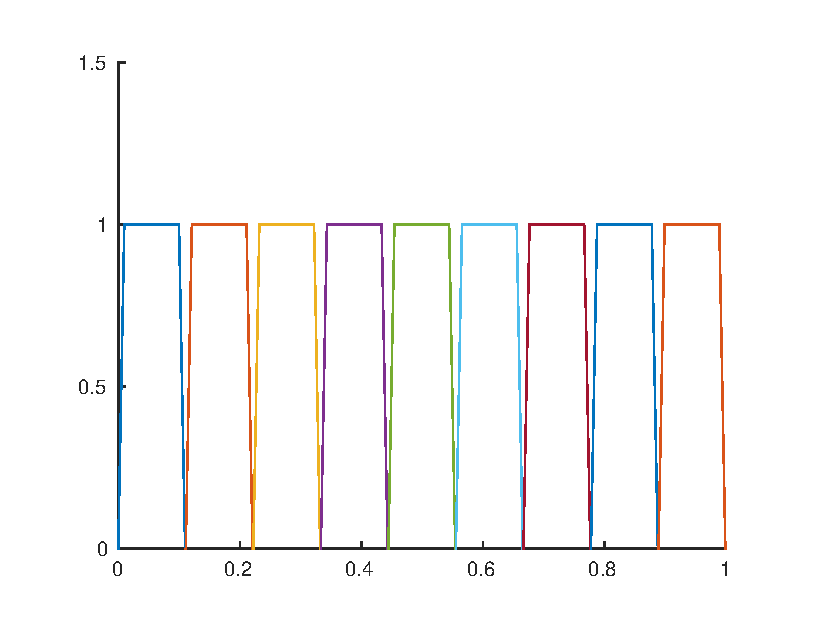
\includegraphics[width=\linewidth]{Pictures/basisconstant}
  \subcaption{B-spline basis for $p=0$}
  \label{fig:bspline_basis_constant}
\end{subfigure}%
\begin{subfigure}[b]{.3\linewidth}
  \includegraphics[width=\linewidth]{Pictures/basislinear}
  \subcaption{B-spline basis for $p=1$}
  \label{fig:bspline_basis_linear}
\end{subfigure}
\begin{subfigure}[b]{.3\linewidth}
  \includegraphics[width=\linewidth]{Pictures/basisquadratic}
  \subcaption{B-spline basis for $p=2$}
  \label{fig:lognorm_quadratic}
\end{subfigure}
\caption{B-spline basis functions, of degree $p=0$ (left), $p=1$ (middle) and $p=2$ (right).}
\label{fig:bsplineBases}
\end{figure}


By giving each of these basis functions a weight $\omega_i$ and normalizing them at each point by dividing by the total sum, we get the rational basis functions. Writing them out explicitly, in terms of B-spline basis functions $N_{i,p}$, the $n^{\text{th}}$-degree NURBS surface with $k$ control points $P_i$ is finally given by:
\begin{equation}
\label{eq:nurbscurve}
\vec{C}(u) = \frac{\sum_{i=1}^{k}N_i^n\left(u\right)\omega_{i}\vec{p}_{i}}{\sum_{i=1}^{k}N_i^n\omega_{i}}.
\end{equation}

B-splines have the following properties, which are useful for our problem:
\begin{itemize}
\item Degree $n$ and number of control points $\vec{P}_{i\cdots m}$ are independent.
\item B-Splines only change locally (depending on the degree $n$) when a control point is changed.
\end{itemize}

Analogous to the tensor product \Bez curve surfaces (see \autoref{eq:bezsurface}), one can define tensor product B-spline or NURBS surfaces:
\begin{equation}
\label{eq:nurbssurface}
\vec{S_\text{NURBS}}(u,v)=\frac{\sum\limits_{i=0}^n \sum\limits_{j=0}^m N_{i}^n(u) N_{j}^m(v) \omega_{i,j}\vec{p}_{i,j}}{\sum\limits_{i=0}^n \sum\limits_{j=0}^m N_{i}^n(u) N_{j}^m(v) \omega_{i,j}},
\end{equation}
where the case with all $\omega_{i,j} = 1$ corresponds to a B-Spline surface; respectively a NURBS surface if any $\omega_{i,j} \neq 1 $. With varying degrees and number of control points, these can be made to fit a variety of shapes. However, as the parameters $u$ and $v$ define a square in their two-dimensional parameter domain, there is a limit to what topologies may be realized with just one such NURBS surface. For example, an open cylinder could be constructed by one such surface where one of the sides meets its own beginning, whereas something with multiple holes - like a double torus, or a non-flat 8-shaped surface, would be impossible. Therefore, when using NURBS, surfaces are most often modelled using a network of connected patches. \todointern{maybe should include an example picture here} For more information about NURBS, see \cite{farin1999nurbs}.



